%\section{Physical Human Factors Report: Tristan Griffith}
\rhead{\today}
\begin{center}
{\large  Tristan Griffith}\\
\vspace{2mm}
{\large Dr. James Hubbard Jr.}
\noindent\rule{\textwidth}{2pt}
\end{center}
\setcounter{section}{1}

%\begin{wrapfigure}{r}{0.45\textwidth}
%\centering
%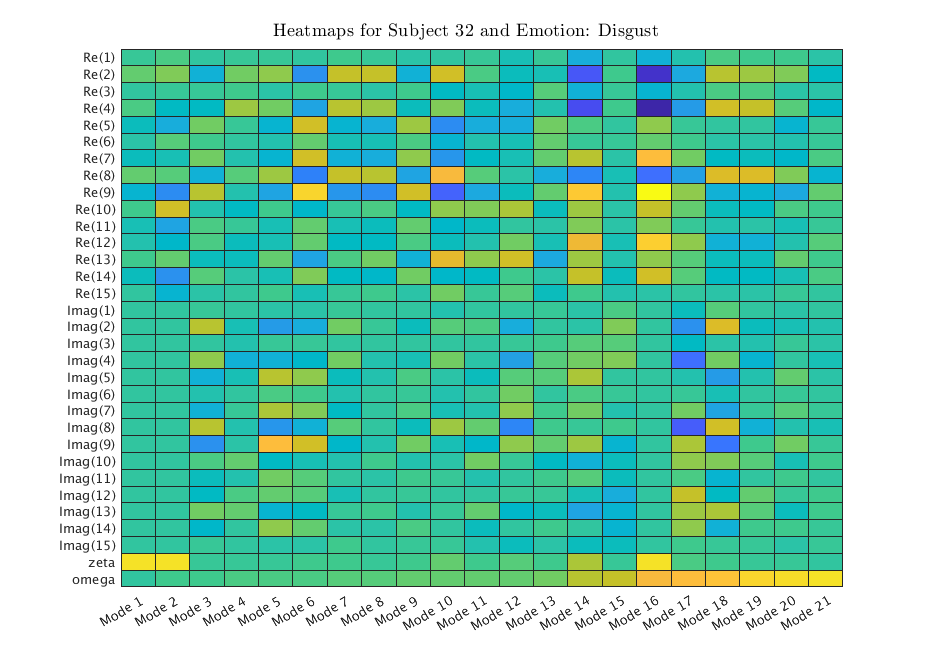
\includegraphics[scale=.3]{../../../figures/demo_map.png} 
%\caption{Modal Heatmap for Subject 32}
%\end{wrapfigure}
\subsection{Motivation}
In the past months, we have become very comfortable converting EEG signals into state space models using output only system identification techniques. As it stands, these models are somewhat useful for biometric classification and analysis, but have not been extended to the quantum domain, which is a desired outcome of our research. The principle barrier preventing the application of quantum probability to these models is the restrictive formulation of the quantum Hilbert space itself, which among other things, requires the state matrix to take the form $-iH$, where $H$ is a self-adjoint matrix. The self-adjoint structure is especially important in quantum probability, because it preserves the norm of the initial condition $\big(||x_0||=||x(t)||\big)$ as the system evolves, ensuring the state vector is still a probability distribution over the possible collapse states.

Physical systems of the form $\dot{x}=Ax+Bu $ rarely have this much structure in their state matrices, so modern system identification techniques do not provide means to directly estimate a self-adjoint matrix from a set of black box measurements. An additional technique is required to convert models generated from these system identification techniques to quantum models robustly, with minimal loss of information. We previously found that generating the self-adjoint matrix as $A_h=\frac{1}{2}(A \pm A^T)$  was removing as much as half the information in the original matrix $A$ as measured by the induced metric. 
\subsection{Problem Statement}
Modern system identification techniques do not allow for the discovery of quantum-like models as the eigenvalues identified from the black box system are not restricted to quantum eigenvalues. Therefore, additional methods are needed to convert these existing system identification state space models into quantum state space models with the accompanying mathematical structure.
\subsection{The Hadamard Transform Applied to EEG Modes}
\subsubsection{Transform Basics}
\label{sec:basics}
The Hadamard transform is the most common method for decomposing signals into a set of orthogonal functions that are not trigonometric which are a specific form of Walsh function. The Hadamard transform is analogous to the Fourier transform, but uses orthogonal square waves instead of sines and cosines. A comparison of the first eight Fourier functions and first eight Hadamard functions is in Figure \ref{fig:hf_comp}.
\begin{figure}[]
    \centering
    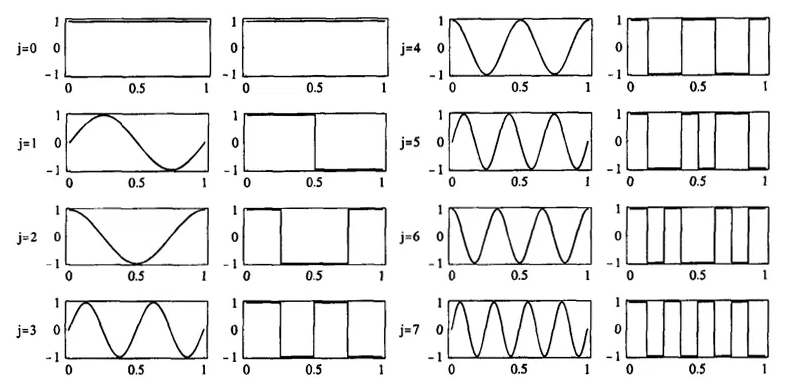
\includegraphics[scale=0.5]{../../../figures/func_comp.png} 
    \caption{Fourier vs. Hadamard Base Functions}
    \label{fig:hf_comp}
\end{figure}
The Hadmard transform has been popular in algorithmic applications, because the nature of square waveforms can be described by a recursive relationship that is easily carried out by computers. The Hadamard transform requires less computational complexity to decompose a given signal into its Walsh functions. The Hadamard transform may be computed with the following recursive function:
\begin{align}
H_1 &\equiv \frac{1}{\sqrt{2}}\begin{bmatrix}
1 & 1\\ 1 & -1
\end{bmatrix} \label{eqn:hada1} \\
H_n=H_1 \otimes H_{n-1}=&\frac{1}{\sqrt{2}}\begin{bmatrix}
H_{n-1} & H_{n-1}\\ H_{n-1} & -H_{n-1}
\end{bmatrix}
\end{align}
Intuitively, equation \ref{eqn:hada1} represents the first two functions in the Walsh function set for the Hadamard transform. The first is a straight line with value one. It has no transition across the origin from 1 to -1, so it does not have any sign changes in its column. The second column corresponds to a function with a single transition from 1 to -1, represented by a single sign change in the column. Higher and higher order Hadamard transforms can be easily determined. The Hadamard matrix corresponding to Figure \ref{fig:hf_comp} is:
\begin{align}
H_8=\left(\begin{array}{cccccccc} 1 & 1 & 1 & 1 & 1 & 1 & 1 & 1\\ 1 & -1 & 1 & -1 & 1 & -1 & 1 & -1\\ 1 & 1 & -1 & -1 & 1 & 1 & -1 & -1\\ 1 & -1 & -1 & 1 & 1 & -1 & -1 & 1\\ 1 & 1 & 1 & 1 & -1 & -1 & -1 & -1\\ 1 & -1 & 1 & -1 & -1 & 1 & -1 & 1\\ 1 & 1 & -1 & -1 & -1 & -1 & 1 & 1\\ 1 & -1 & -1 & 1 & -1 & 1 & 1 & -1 \end{array}\right) \label{eqn:h8}
\end{align}
Notice that the ordering of the columns in equation \ref{eqn:h8} is not ordered from least to most transitions, but that the constant 1 function is immediately followed by the square wave with the maximum number of transitions. These columns may be reordered for convenience or interpretation. Ordering in terms of number of transitions is known as sequency ordering, as in Figure \ref{fig:hf_comp}, and is most commonly found in signal processing applications.  Hadamard ordering, which is used in controls applications, arranges them as 0, 4, 6, 2, 3, 7, 5, 1. Dyadic or gray code ordering, which is used in mathematics, arranges them as 0, 1, 3, 2, 6, 7, 5, 4.
\begin{figure}[]
    \centering
    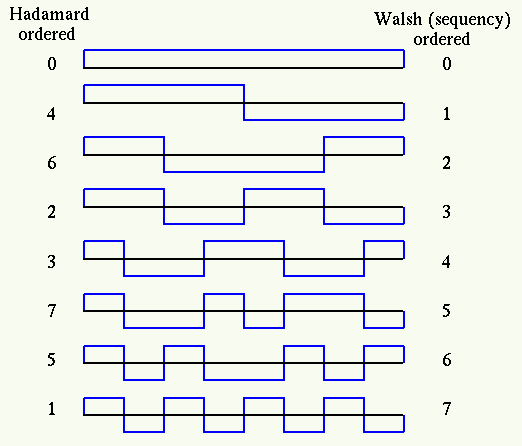
\includegraphics[scale=0.5]{../../../figures/wht_waveform_1.png} 
    \caption{Hadamard vs. Sequency Ordering}
    \label{fig:ordering}
\end{figure}
Keeping track of which ordering method an algorithm uses is critical. The Discrete Walsh Hadamard Transform (DWHT) had been widely used for biometric identification, data compression, and image segmentation. Figure \ref{fig:comp} demonstrates how the DWHT, along with the Discrete Cosine Transform (DCT), are better suited to image compression that traditional methods centered on the Discrete Fourier Transform (DFT) \cite{bull2014communicating}.
\begin{figure}[]
    \centering
    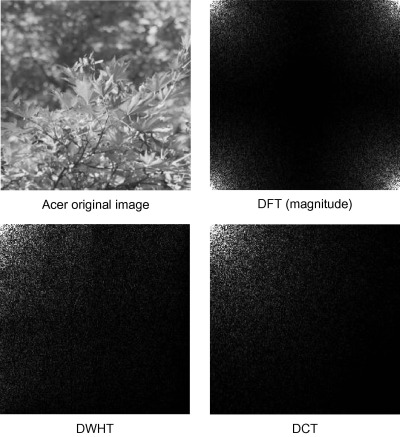
\includegraphics[scale=0.7]{../../../figures/hada_example.jpg} 
    \caption{Comparison of Decomposition Methods}
    \label{fig:comp}
\end{figure}
Notice that the DWHT and DCT concentrate their high energy areas in a single corner, unlike the DFT. This makes it much easier to set a cutoff point for image compression. 
\subsubsection{Hadamard Logic Gates}
Nothing in the previous section indicates that the Hadamard transform is better suited to application on quantum cognitive models than any other decomposition method. The Hadamard transform piqued our interest due to its relevance in both signal processing and quantum logic gate operations. Hadamard Gates are often used as the first step in a proposed quantum algorithm. They have the neat property of smearing the initial condition into a superposition of all possible states evenly in a given quantum probability space.

For example, if we are working in a two dimensional space, such as that of qubits, we may have an initial state:
\begin{align}
x_0=\begin{bmatrix}
1 \\ 0
\end{bmatrix}
\end{align}
If we pass this initial state through a Hadamard Gate, it becomes:
\begin{align}
H x_0=x_0'\\
\frac{1}{\sqrt{2}}\begin{bmatrix}
1 & 1\\1 & -1
\end{bmatrix}\begin{bmatrix}
1 \\ 0
\end{bmatrix}=\frac{1}{\sqrt{2}}\begin{bmatrix}
1 \\ 1
\end{bmatrix}
\end{align}
Before passing the initial condition through the Hadamard gate, the system was in a prepared state. After passing through the gate, the probability distribution is evenly distributed over both possible measurement outcomes. Notice that it is very important to carry the normalizing term along with the Hadamard matrix so that it is a unitary transform. This is true for systems of higher order, of course:
\begin{align}
x_0=\begin{bmatrix}
0 \\ 1 \\ 0 \\0 
\end{bmatrix}\\
x_0'=\frac{1}{2}\left(\begin{array}{cccc} 1 & 1 & 1 & 1\\ 1 & -1 & 1 & -1\\ 1 & 1 & -1 & -1\\ 1 & -1 & -1 & 1 \end{array}\right)\begin{bmatrix}
0 \\ 1 \\ 0 \\0 
\end{bmatrix}=\frac{1}{2}\begin{bmatrix}
1 \\ -1 \\1\\-1
\end{bmatrix}
\end{align}
And so on and so on. For algorithms where we expect a certain outcome regardless of initial conditions, this is a quick method to remove potential bias in the preparation of the quantum state. Notice further that this process is reversible, and we can recover $x_0$ from $x_0'$.
\subsubsection{``Quantumness'' of OMA and Hadamard Modes}
So we've established an intuitive connection to the Hadamard transform. It's useful in signal processing and in quantum probability, so it may get us closer to a probabilistic model of cognition. We may look at the resultant state space model from our operational modal analysis on EEG data $A_{OMA}$. $A_{OMA}$ has complex eigevalues and eigenvectors. Further, the eigenvectors are not orthogonal. Quantum state Hamiltonian matricies are known to have only real valued eigenvalues with corresponding orthogonal eigenvectors which represent the basic observables in the quantum model. We may Hadamard transform $A_{OMA}$:
\begin{align}
A_{h}=HA_{OMA}
\end{align}
The resultant matrix has real valued eigenvalues, which gets us a little closer to a quantum Hamiltonian. Regardless of the ordering, however, the eigenvectors of $A_h$ are not orthogonal unless the original eigenvalues of $A_{OMA}$ were orthogonal to begin with. 

A computational example illustrates this point. The identify matrix has orthogonal eigenvectors beforehand:
\begin{align}
\phi_0(I)=\begin{bmatrix}
1 \\0
\end{bmatrix},\begin{bmatrix}
0 \\ 1
\end{bmatrix}\\
I_{h}=HI\\
I_{h}=\frac{1}{\sqrt{2}}\begin{bmatrix}
1 & 1\\1 & -1
\end{bmatrix}\begin{bmatrix}
1 & 0\\0 & 1
\end{bmatrix}\\
\lambda_{I_h}=\pm 1\\
\phi=\begin{bmatrix}
1 \pm \sqrt{2} \\ 1
\end{bmatrix}
\end{align}
While $I_h$ has different eigenvectors than $I$, they remain orthogonal. Conversely, if we consider an example 2x2 matrix from our OMA analysis:
\begin{align}
A_{OMA}=\left(\begin{array}{cc} 0.728 & 0.345\\ -0.378 & 0.923 \end{array}\right)\\
\phi_0(A_{OMA})=\left(\begin{array}{cc} 0.186-0.665{}\mathrm{i} & 0.186+0.665{}\mathrm{i}\\ 0.723 & 0.723 \end{array}\right) \label{eqn:phiA}
\end{align}
From equation \ref{eqn:phiA}, it can be seen that the eigenvectors are not orthogonal.
\begin{align}
A_{h}=HA_{OMA}\\
A_{h}=\frac{1}{\sqrt{2}}\begin{bmatrix}
1 & 1\\1 & -1
\end{bmatrix}A_{OMA}\approx \left(\begin{array}{cc} 0.248 & 0.896\\ 0.782 & -0.409 \end{array}\right)\\
\lambda_{A_h}=0.819,-0.980\\
\phi(A_h)=\left(\begin{array}{cc} 0.843 & -0.59\\ 0.537 & 0.808 \end{array}\right)
\end{align}
A few things to note here:
\begin{itemize}
\item Neither $A_{OMA}$, or $A_h$ have orthogonal eigenvectors
\item $A_h$ has eigenvalues in the right half plane (unstable poles)
\item Unlike $A_{OMA}$, notice that $A_h\approx A_h^*$
\end{itemize}
Therefore, we have to conclude that the Hadamard transform doesn't get us all the way to a quantum Hamiltonian. However, I notice that it provides wholly real eigenvalues, which is a step closer to quantum. Further, the state matrix is almost self-adjoint, and looks to me like some of the noisy state matrices I used to develop the earlier \href{https://drive.google.com/file/d/17kZl22Yy5hwzDv9F1psR9IAmViYwAzik/view?usp=sharing}{least squares SINDy like Hamiltonian estimator}. Perhaps we can go one more step, using the SINDy algorithm to get to a quantum Hamiltonian. 
\subsubsection{Least Squares to Nearest Hamiltonian}
So far, we've shown that the Hadamard transform, while getting us closer to a quantum Hamiltonian, does not totally complete the path from EEG signals to quantum probability space. 

\textcolor{red}{Ok. So this was a nice idea. I could be further developed. However, as I'm looking at the linear systems side of things, we have issues.} Primarily, with the transform taking the form $A_{h}=HA_{OMA}$, the transform is operating on the state matrix, not on the vector. Normally a transform is defined as:
\begin{align}
\bar{x}=Tx\\
\bar{\dot{x}}=T\dot{x}\\
\dot{x}=Ax\\
T^{-1}\bar{\dot{x}}=AT^{-1}\bar{x}\\
\bar{\dot{x}}=TAT^{-1}\bar{x}\\
\end{align}
However, I did something different:
\begin{align}
\bar{x}=HA\dot{x}
\end{align}
Since the operation was applied on the state matrix and not on the state vector, the thing you are differentiating in $\dot{x}$ and the result of $\bar{x}$ aren't the same. After consulting with Dr. Balas (2020-11-05), I'm not aware of other transforms like that, and I've destroyed the meaning or use of the state transition matrix $\Phi$. Even though $\bar{x}$ is in a quantum space, $\dot{x}$ is still in the measure space. I may abandon this for the time being and take a look at some other methods. Argh so close. 
\subsubsection{Reachability?}
I would have shown that the use of the least squares estimator averages the distance between the off diagonal components, and that introduces an interval for reachability. 
\subsection{Results}
\subsubsection{A Quantum Hamiltonian}
\subsubsection{Interpretation of Model}

\subsection{Discussion}




%\begin{displayquote}
%The class of monotone DNF expressions is learnable via an algorithm $B$ that uses $L=L(h,d)$ calls of examples and $dt$ calls of oracle, where $d$ is the degree of the DNF expression $f$ to be learnt and $t$ the number of variables.
%\end{displayquote}


%\begin{wrapfigure}{r}{0.55\textwidth}
%\centering
%\includegraphics[scale=.5]{../figures/complexity.png} 
%\caption{The Error-Complexity Trade Off}
%\end{wrapfigure}

